\section{Problem 3}
\label{part3}
\begin{verbatim}
Estimate the age of each of the 1000 URIs using the "Carbon Date" tool:

http://ws-dl.blogspot.com/2013/04/2013-04-19-carbon-dating-web.html

Note: you'll have better luck downloading and installing the tool 
rather than using the web service (which will run slowly and likely
be unreliable).

For URIs that have > 0 Mementos and an estimated creation date,
create a graph with age (in days) on one axis and number of mementos
on the other.

\end{verbatim}
\subsection{Solution}
\begin{enumerate}

\item Downloaded the carbon tool provided and installed as instructed in the readme file. 
\item From some test runs, it became apparent that the Carbon Date tool takes between 1 and 7 minutes to query all of its services for a given URI. 
\item So getting the dates for all the 1000 URI's from a single script will take more than 36 hours so i executed 5 scripts in 5 different Linux servers which let me extract all the links in 12 hours. 
\item Made changes to local.py from the carbon tool 
in order to read 1000 URI's from a text file and write back the result(time,URI) into an other text file
\item Getting the dates was not enough, because we need the age of each link. 
\item I have written a small python program(caldays.py) which will take the date got from the Carbon Date tool and calculated the days 
\item We will have to create a graph for the links which have >0 mementos and the days for that link
\item So inorder to filter the links which have mementos>0 and get the days, i have written an other simple python program  memvsdays.py.
\item memvsdays.py will collect the data which we need to build a graph for URIs that have > 0 Mementos and the days . 

\end{enumerate}
\newpage
\subsection{Code Listing}

\subsubsection{local.py}
\lstinputlisting[language=Python,breaklines = true,frame=single,caption={Python program for getting creation date for URI's}, label=lst:q1-1,captionpos=b,numbers=left,showspaces=false,showstringspaces=false,basicstyle=\footnotesize]{local1.py}
\newpage
\subsubsection{cladays.py}
\lstinputlisting[language=Python,breaklines = true,frame=single,caption={Python program for calculating the age of URI's}, label=lst:q1-1,captionpos=b,numbers=left,showspaces=false,showstringspaces=false,basicstyle=\footnotesize]{caldays.py}
\newpage
\subsubsection{memvsdays.py}
\lstinputlisting[language=Python,breaklines = true,frame=single,caption={Python program for collecting Mementos versus days}, label=lst:q1-1,captionpos=b,numbers=left,showspaces=false,showstringspaces=false,basicstyle=\footnotesize]{memvsdays.py}
\subsubsection{q3graph.R}
\lstinputlisting[language=R,breaklines = true,frame=single,caption={R program for generating the histograms for Question 2}, label=lst:q2R,captionpos=b,numbers=left,showspaces=false,showstringspaces=false,basicstyle=\footnotesize]{q3graph.R}
\newpage
\subsection{Results}
\subsubsection{carbondates.txt}

\verbatiminput{samplelinks.txt}

\newpage
\subsubsection{carbonday.txt}

\verbatiminput{carbondates.txt}
\newpage
\subsubsection{memvsday.txt}
\verbatiminput{memvsday.txt}
\newpage
\subsubsection{q3-scatterplot}
\begin{figure}[ht]    
    \begin{center}
        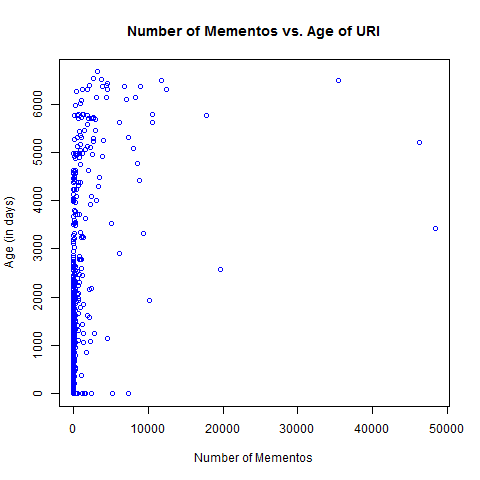
\includegraphics[scale=0.60]{q3-scatterplot.png}
        \caption{ScatterPlot}
        \label{scatterPlot}
    \end{center}
\end{figure}